% !TeX spellcheck = cs_CZ
\wikitextrule
\begin{example}\label{mai:exam075}
  \textbf{Záhada přijímací zkoušky aneb k čemu může posloužit distribuční funkce?}\newline\small
  Mohlo by se zdát, že distribuční funkce je jen teoretický pojem a že v praktických situacích ji 
  těžko využijeme. Podstatné je přece pravděpodobnostní rozdělení náhodné veličiny a distribuční 
  funkce je z něj jen jaksi odvozena sčítáním pravděpodobností (u diskrétního rozdělení) nebo 
  integrací (u rozdělení spojitého). Přesvědčíme se, že existují velmi realistické případy, kdy 
  distribuční funkce přináší věrohodnější informaci o náhodné veličině než samotné rozdělení.
  
  Na Masarykově univerzitě musí každý uchazeč o studium, ať již se hlásí na přírodovědeckou, 
  právnickou, lékařskou či jinou fakultu, absolvovat Test studijních předpokladů. Jedná se o 
  všeobecný test, zaměřený na zjišťování úrovně všech schopností uchazeče, které jsou potřebné pro 
  univerzitní studium, například analytického myšlení, verbálních schopností, numerického myšlení, 
  geometrické představivosti, atd. Pro nás však v tu to chvíli není podstatný obsah testu, ale 
  způsob zpracování jeho výsledků a vyhodnocení pořadí uchazečů. Test skládá kolem třiceti tisíc 
  studentů. Není tedy možné technicky zajistit, aby proběhl v jediné variantě v jednom dni.
  K dispozici je proto osm variant testu, každou variantu řeší tři až čtyři tisíce studentů. Test 
  má \num{80} otázek, základním údajem pro zpracování jeho výsledků je počet správných odpovědí 
  každého studenta. Pokud bychom označili jako \(i\) počet správných odpovědí (\(i \in\lbrace0, 1, 
  2, \ldots, 80\rbrace\)) v kterékoli variantě a \(\mathcal{N}_i\) počet studentů, kteří
  dosáhli právě \(i\) správných odpovědí, dostaneme náhodnou veličinu \(X_i\), kterou bychom mohli 
  nazvat „počet správných odpovědí“, pro celou univerzitu. Její rozdělení by mělo tvar
  \begin{equation*}
    \lbrace(i,p_i)\rbrace,\qquad\text{kde}\qquad p_i = \dfrac{\mathcal{N}_i}{\mathcal{N}}, \qquad
    \mathcal{N} = \sum_{i=0}^{80}\mathcal{N}_i
  \end{equation*}
  A zde je malý „kámen úrazu“. A by bylo možné sestavit opravdu „univerzální pořadí“, musely by být 
  všechny varianty testu ekvivalentní z hlediska obtížnosti. To znamená, že kdyby kterýkoli student 
  vyplnil za stejných podmínek všechny varianty, dosáhl by v každé z nich stejného počtu správných 
  odpovědí s pravděpodobností velmi blízkou jedné. Skutečnost je však principiálně taková, že u 
  sebelépe promyšleného a sestaveného testu se jednotlivé varianty budou mírně, v rámci 
  statistických, a tedy již neodstranitelných, odchylek lišit. Tato odlišnost se nepozná předem, 
  ale až po zpracování výsledků všech variant. Použít pro stanovení pořadí uchazečů rozdělení
  náhodné veličiny \(X\) \emph{= počet správných odpovědí je tedy nespravedlivé}. Student, který 
  řešil variantu „statisticky obtížnější“, by v pořadí skončil s horším umístěním, než student, 
  který je stejně schopný, avšak měl to štěstí, že na něj připadla varianta „statisticky méně 
  obtížná“. Skutečně, kdybychom sestavili grafy rozdělení náhodných veličin \(X^{(\alpha)}\) 
  \emph{= počet správných odpovědí v \(\alpha\)-té variantě},
  \begin{equation*}
    \lbrace(i,p_i^{(\alpha)})\rbrace,\qquad\text{kde}\qquad 
    p_i^{(\alpha)} = \dfrac{\mathcal{N}_i^{(\alpha)}}{\mathcal{N}^{(\alpha)}}, \qquad
    \mathcal{N}^{(\alpha)} = \sum_{i=0}^{80}\mathcal{N}_i^{(\alpha)}
  \end{equation*}
  zjistili bychom, že se mírně liší. (V předchozím zápisu značí \(\mathcal{N}_i^{(\alpha)}\) počet 
  studentů, kteří odpověděli správně na \(i\) otázek \(\alpha\)-té varianty 
  \(\mathcal{N}^{(\alpha)}\) je počet všech studentů, kteří tuto variantu řešili.) Střední hodnoty 
  i mediány náhodných veličin se i při vynikající shodě obtížnosti všech variant mohou lišit v 
  rozmezí jedné až dvou správných odpovědí. A s ohledem na skutečnost, že každou variantu řeší 
  obrovský počet studentů, až čtyři tisíce, je zřejmé, že tento rozdíl může poněkud „zamíchat“ 
  pořadím, zejména v blízkosti mediánu, kde se týká třeba i tří stovek studentů v každé variantě. 
  Situaci dokládá obrázek \ref{mai:fig049}. Jak tedy zařídit, abychom dostali spravedlivé pořadí? 
  Jediný rozumný způsob, jak minimalizovat vliv statistických odchylek obtížnosti jednotlivých 
  variant, je nehodnotit studenty podle absolutního počtu správných odpovědí, ale nějak je porovnat 
  mezi sebou. Budeme při tom předpokládat, že rozložení schopností studentů je ve všech osmi 
  skupinách, které řeší osm daných variant, stejné. Řeknete si — zase nějaké další předpoklady. To 
  je jako z bláta do louže. Předpoklad o stejném rozložení schopností studentů v tak velkých 
  skupinách, jako jsou ty naše, je však mnohem realističtější než předpoklad o dokonalé shodě 
  obtížnosti variant testu. Budeme se jej proto držet. Každému studentovi přisoudíme číslo,
  které informuje o tom, kolik řešitelů dané varianty bylo horších nebo stejně dobrých jako on, tj. 
  mělo nižší nebo stejný počet správných odpovědí. Z matematického hlediska to znamená přejít v 
  každé variantě od rozdělení k distribuční funkci. Věnujme se nyní tomuto přepočtu podrobněji jak 
  pro diskrétní rozdělení náhodné veličiny \(X^{(\alpha)}\), které odpovídá skutečné situaci, tak 
  pro zajímavost i pro rozdělení spojité. V dalším budeme vždy zpracovávat výsledky jedné varianty, 
  upustíme proto od vyznačování indexu \(\alpha\).

  {\centering
   \captionsetup{type=figure}
   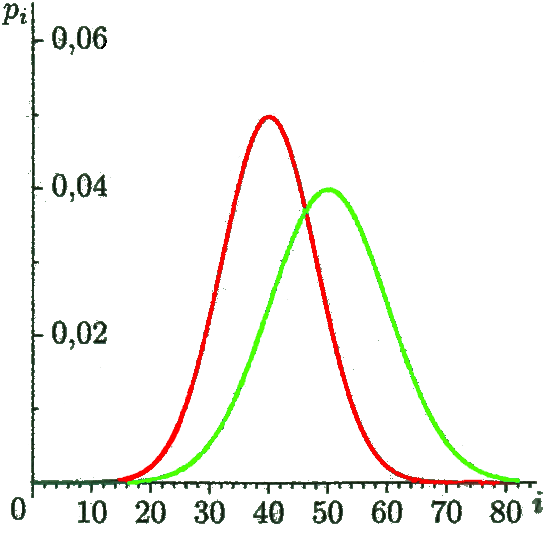
\includegraphics[width=0.4\linewidth]{mai_fig049.png}
   \captionof{figure}{Rozdělení pro dvě varianty testu,
   \cite[s.~252]{Musilova2009MA1}
   \label{mai:fig049}}
  \par}
  
  \textbf{Diskrétní rozdělení}
    \begin{itemize}
      \item \emph{Zadání:} Skupina \(N\) studentů řeší jednu variantu testu. Test má \(Q\) otázek. 
            Za každou správnou odpověď je přidělen jeden výchozí bod. Získáváme rozdělení
            \begin{equation*}
              \left\lbrace\left(i, \dfrac{N_i}{N} \right)\right\rbrace, \qquad
              i\in\lbrace0, 1, 2, \ldots, Q\rbrace, \qquad
              \sum_{i=0}^{Q}N_i = N 
            \end{equation*}
            kde \(i\) je počet výchozích bodů a \(N_i\) počet studentů, kteří získali \(i\) bodů. 
            Distribuční funkce tohoto rozdělení
            \begin{equation*}
              F(x) = \dfrac{1}{N}\sum_{i=0}^{j}N_i\qquad\text{ pro }\qquad
              j\leq x < j+1, \qquad x\in\left[0,\infty\right)
            \end{equation*}
            Pro uchazeče, který získal \(j\) bodů, mají význam následující hodnoty:
            \begin{itemize}
              \item \(F(x)    x \in \left[j, j+1\right)\): poměrný počet uchazečů, kteří 
                    získali počet výchozích bodů nižší nebo shodný s daným uchazečem,
              \item \(NF(x)   x \in \left[j, j+1\right)\): absolutní počet uchazečů, kteří získali 
                    počet výchozích bodů nižší nebo shodný s daným uchazečem,
              \item \(100F(x) x \in \left[j, j+1\right)\): absolutní počet uchazečů, kteří získali 
                    počet výchozích bodů nižší nebo shodný s daným uchazečem,
            \end{itemize}
      \item Hodnoty distribuční funkce můžeme získat z následující tabulky:
            \begin{table}[ht!]
              \centering
              \resizebox{0.4\textwidth}{!}{%
              \begin{tabular}{c|c}
                        interval \(x\)     &  \(NF(x)\)         \\ \hline
                \(\left[0,1\right)\)       &  \(N_0\)           \\ 
                \(\left[1,2\right)\)       &  \(N_0 + N_1\)     \\ 
                \(\cdots\)                 &  \(\cdots\)        \\
                \(\left[j,j+1\right)\)     &  \(N_0 + N_1 + \cdots + N_j\)           \\ 
                \(\cdots\)                 &  \(\cdots\)                             \\
                \(\left[Q-1,Q\right)\)     &  \(N_0 + N_1 + \cdots + N_{Q-1}\)       \\ 
                \(\left[Q,\infty\right)\)  &  \(N_0 + N_1 + \cdots + N_{Q} = N\)     \\ 
              \end{tabular}}
              % \caption{ }
            \end{table}
      \item Přepočet hodnocení uchazečů tak, aby nová stupnice byla opět v rozsahu mezi nulou a 
            \(Q\) a aby nové hodnocení bylo opět celočíselné, je následující:
            \begin{equation*}
              y =QF(x), \qquad 0\leq F(x) \leq 1, \Rightarrow y \in[0,Q].
            \end{equation*}
            Uchazeči se ziskem \(i\) výchozích bodů náleží hodnota \(y = QF(x)\) právě když i\( \in 
            \left[i, í + 1\right)\), tj. \(y_i = Q F(i)\). Tato hodnota není obecně celočíselná. 
            Zaokrouhlení se provede ve prospěch uchazeče, tedy vždy nahoru. Výsledný převodní 
            vzorec je
            \begin{equation*}
              \text{výchozí body } i \longrightarrow\text{ nové body } Y_i: Y_i = [y_i] + 1 = 
              [QF(i)] + 1,
            \end{equation*}
            kde \([a]\) značí celočíselnou část čísla \(a\), tedy například \([\num{23.05}] = 
            [\num{23.48}] = [23,89] = 23\)
      \item Zaveďme novou náhodnou veličinu \(Z\) s rozdělením \(\left\lbrace(z_\alpha, 
            M_\alpha)\right\rbrace\): Označme \(z_1, z_2, \ldots, z_\alpha, ...,\) \(z_S\) navzájem
            různé hodnoty ze souboru \(\lbrace Y_i\rbrace, i = 0, 1, 2, \ldots, Q\) řazené 
            vzestupně. Její rozdělení udává kterákoli z následujících tabulek:
            \begin{table}[ht!]
              \centering
              \resizebox{0.5\textwidth}{!}{%
              \begin{tabular}{c|c}
                        hodnota                       &  četnost         \\ \hline
                \(z_1 = Y_0 = Y_1 = \cdots Y_{i_1}\)  &  \(M_1 = N_0 + N_1 + \cdots + N_{i_1}\)  \\ 
                \(Z_2 = Y_{i_1+1} = \cdots Y_{i_2}\)  &  \(M_2 = N_{i_1+1} + \cdots + N_{i_2}\)  \\ 
                \(\cdots\)                            &  \(\cdots\)                              \\
                \(Z_S = Y_{i_{S-1}+1}=\cdots Y_{i_S}\) & \(M_S = N_{i_{S_1}+1}+\cdots+N_{i_S}\)   
              \end{tabular}}
              % \caption{ }
            \end{table}

            \begin{table}[ht!]
              \centering
              \resizebox{0.5\textwidth}{!}{%
              \begin{tabular}{c|c}
                        hodnota                       &  četnost         \\ \hline
                \(z_1 = Y_0 = Y_1 = \cdots Y_{i_1}\)  &  \(M_1 = NF(i_1)\)  \\ 
                \(Z_2 = Y_{i_1+1} = \cdots Y_{i_2}\)  &  \(M_2 = N[F(i_2) - F(i_1)] \)  \\ 
                \(\cdots\)                            &  \(\cdots\)                              \\
                \(Z_S = Y_{i_{S-1}+1}=\cdots Y_{i_S}\) & \(M_S = N[F(i_S) - F(i_{S-1})]\)   
              \end{tabular}}
              % \caption{ }
            \end{table}
            kde \(i_1 < i_2 < \ldots < i_{S-1} < i_S, i_S = Q\) (Vzhledem k zaokrouhlování nahoru 
            není žádná bodová hodnota \(Y_i\) nulová.) I když skutečné rozdělení při zpracování 
            výsledků testů je diskrétní, ukažme si, jak by vypadal analogický postup u rozdělení 
            spojitého, kde je početní zpracování názornější.
    \end{itemize}
  
  \textbf{Spojité rozdělení}
    \begin{itemize}
      \item \emph{Zadání:} Je dáno rozdělení četností \(n(x) \leq 0,\, x \in [0, Q]\).
      \item Normovací podmínka a distribuční funkce jsou
            \begin{equation*}
              \int_{0}^{Q}n(x)\dd{x} = N, \qquad 
              F(x) = \dfrac{1}{n}\int_{0}^{x}n(\xi)\dd{\xi}, \qquad
              0 \leq F(x) \leq 1.
            \end{equation*}
      \item Označme \(z = QF(x)\), tedy \(z \in [0, Q]\), novou náhodnou veličinu. (Uvědomme si, že 
            \(z\) je rostoucí funkcí proměnné \(x\)). Označme její rozdělení \(\nu(z)\). Její 
            distribuční funkce je
            \begin{equation*}
              \Phi(z) = \int_{0}^{z}\nu(\zeta)\dd{\zeta} 
                      = \int_{0}^{x(z)}\dfrac{n(\xi)}{N}\dd{\xi}
                      = F\left(F^{-1}(z/Q)\right) 
                      = \dfrac{z}{Q}, \qquad
              \nu(z) = \dfrac{1}{Q}.
            \end{equation*}
      \item Rozdělení je konstantní s mediánem i střední hodnotou \(Q/2\). Takové rozdělení se 
            nazývá rovnoměrné.
    \end{itemize}
    
  
\normalsize
\end{example}